\chapter{ Констукторский раздел}
\label{cha:design}

Рассмотрим задачу получения видео с динамически расширенным диапазоном из поданного потока данных. 

\section{ Описание метода}

    Особенностью решения данной задачи является то, что исходное видео, подающееся на вход, может быть получено путем ручной съемки. Так как видео материал это не что иное, как последовательность кадров, они могут быть не выровнены по отношению друг к другу, а так же объекты, запечатленные на камеру, могут быть не статичны, что усложняет получение HDR изображения, а следовательно и самого видео. В качестве алгоритма выравнивания(регистрации изображения) был выбран алгоритм MTB\cite{bib4}. Алгоритм для удаления движущихся объектов на последовательности кадров - MBD\cite{bib5}. Так как стоит задача отображения HDR видео на LDR мониторе, наиболее подходящим алгоритмом слияния кадров является алгоритм слияния экспозиций\cite{bib7}. Так же требуется выбирать кадры с разной экспозицией из последовательности кадров(видео). Для алгоритма выделяются основные этапы:

\begin{itemize}
    \item Выбор нужных кадров из видео материала
    \item Выравнивание кадров по отношению друг к другу(MTB алгоритм)
    \item Нахождение артефактов(возникших из-за движущихся объектов)
    \item Получение LDR изображения с расширенным динамическим диапазоном
    \item Объединение полученных кадров в видео ряд и сохранение на устройстве
\end{itemize}

В итоге, вся задача сводится к работе с изображениями.

\section{ Декомпозиция разрабатываемого метода}

Представим задачу получения HDR видео ряда на LDR мониторе в виде диаграммы "IDEF0" на Рисунке \ref{fig:A}, Рисунке \ref{fig:A0}, Рисунке \ref{fig:A2}, Рисунке \ref{fig:A21}, Рисунке \ref{fig:A22}, Рисунке \ref{fig:A23}

\begin{figure}[ht!]
    \centering{
        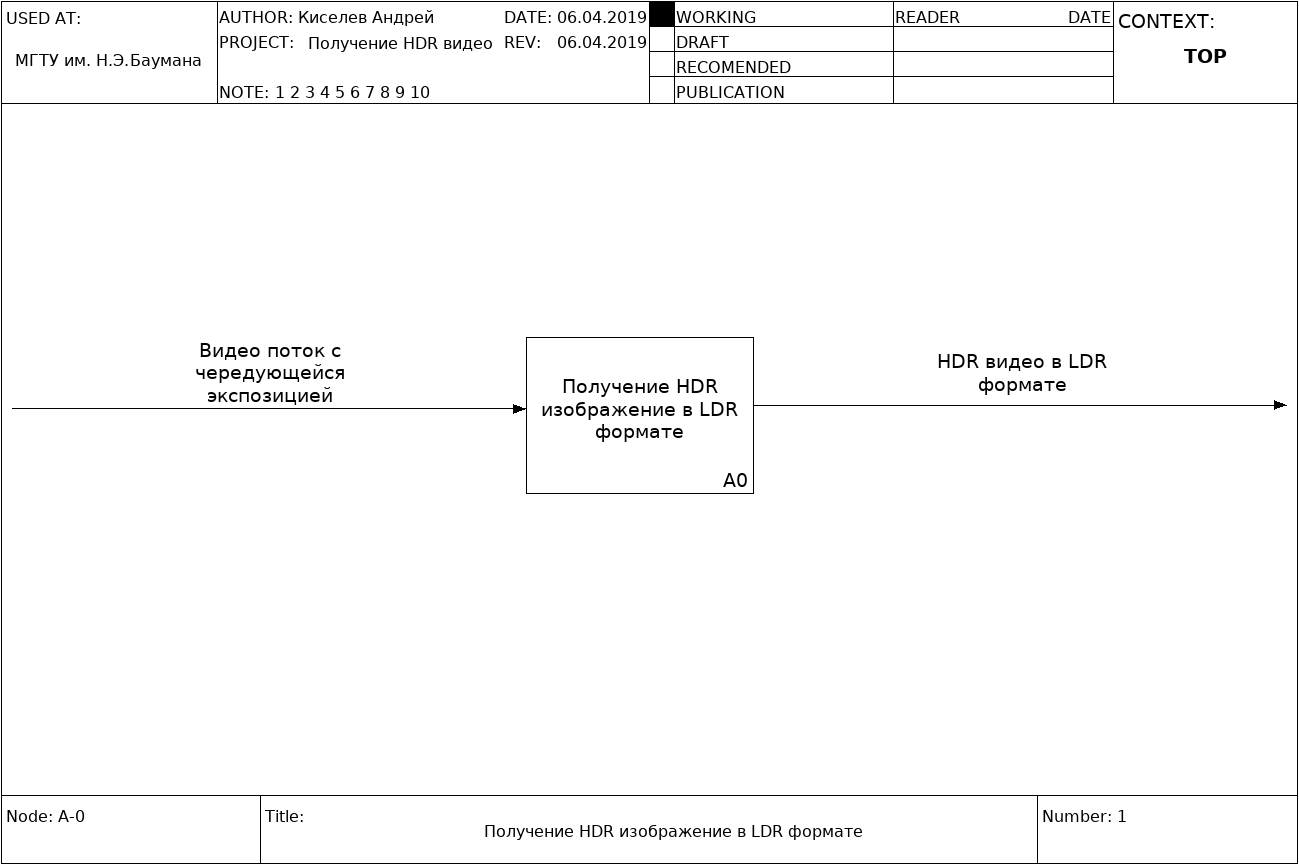
\includegraphics[width=1\textwidth]{img/01_A-0.png}
	\caption{ IDEF0 диаграмма метода(A)}
        \label{fig:A}
        }
\end{figure}

\begin{figure}[ht!]
    \centering{
        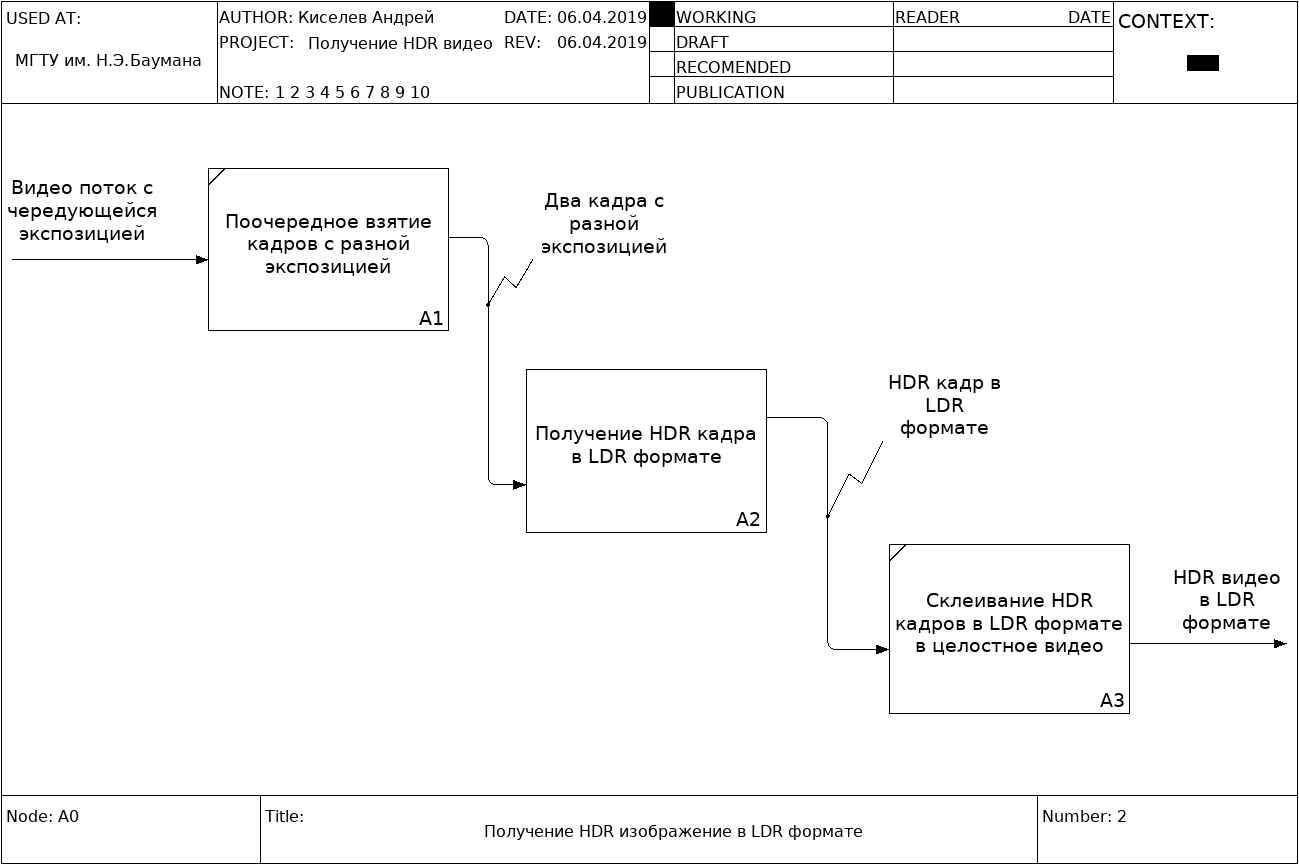
\includegraphics[width=1\textwidth]{img/02_A0.png}
	\caption{ IDEF0 диаграмма метода(A0)}
        \label{fig:A0}
        }
\end{figure}

\begin{figure}[ht!]
    \centering{
        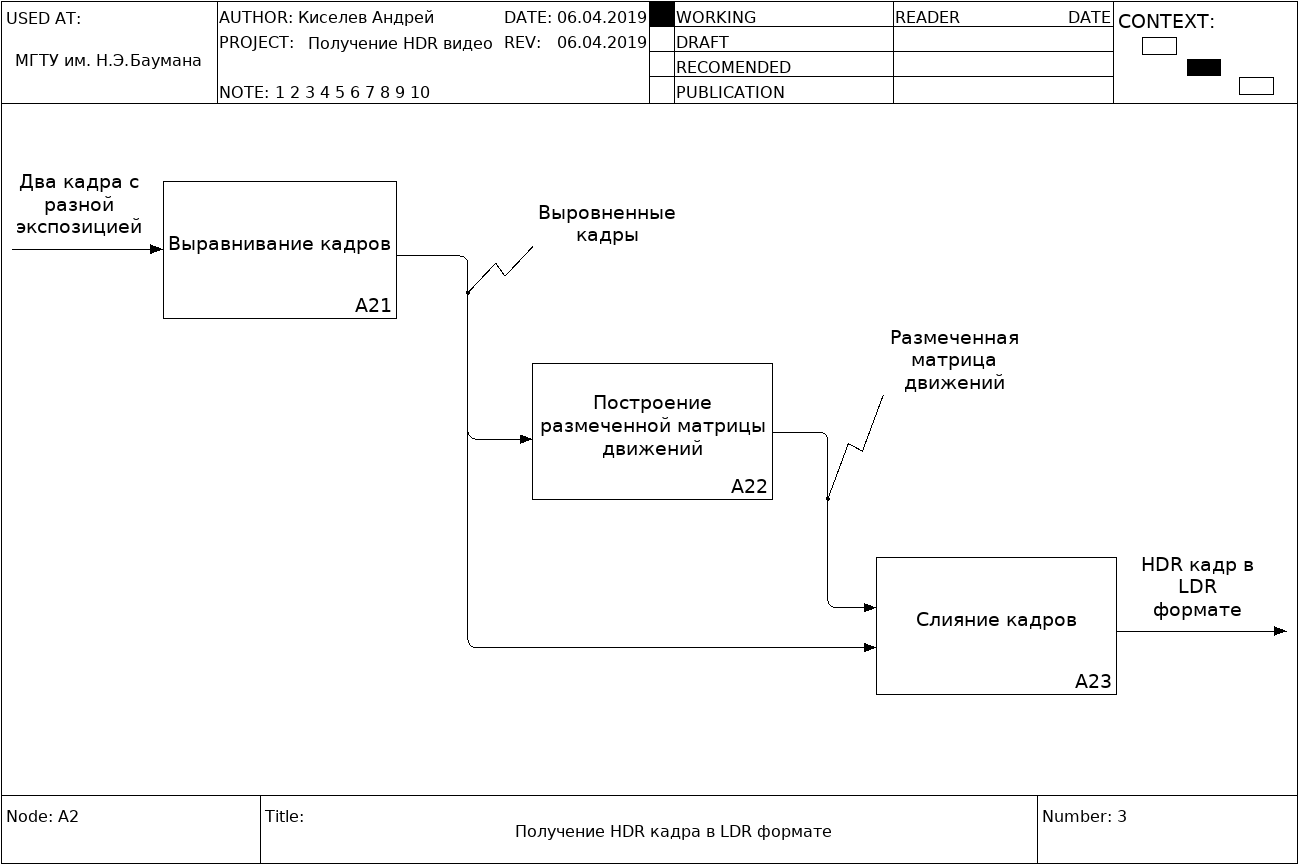
\includegraphics[width=1\textwidth]{img/03_A2.png}
	\caption{ IDEF0 диаграмма метода(A2)}
        \label{fig:A2}
        }
\end{figure}

\begin{figure}[ht!]
    \centering{
        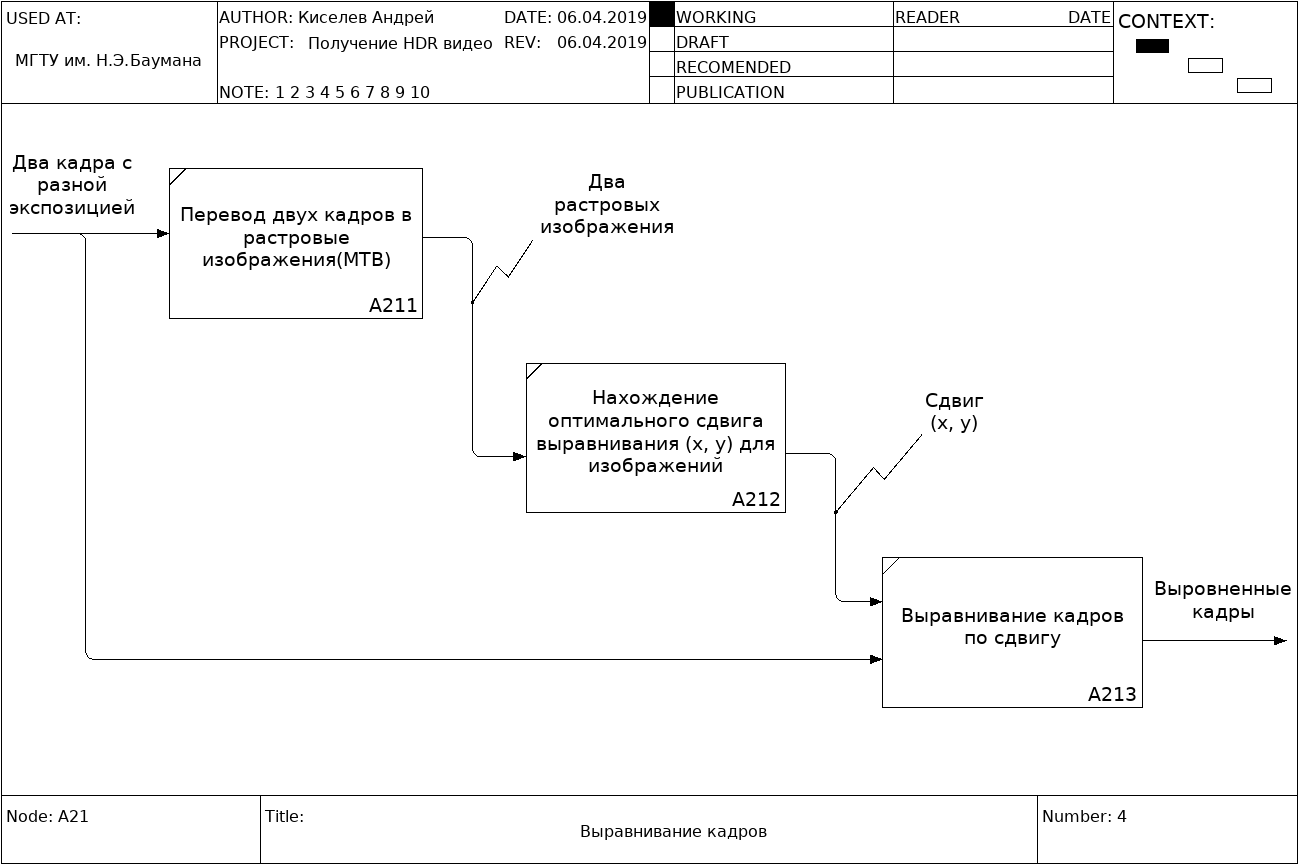
\includegraphics[width=1\textwidth]{img/04_A21.png}
	\caption{ IDEF0 диаграмма метода(A21)}
        \label{fig:A21}
        }
\end{figure}

\begin{figure}[ht!]
    \centering{
        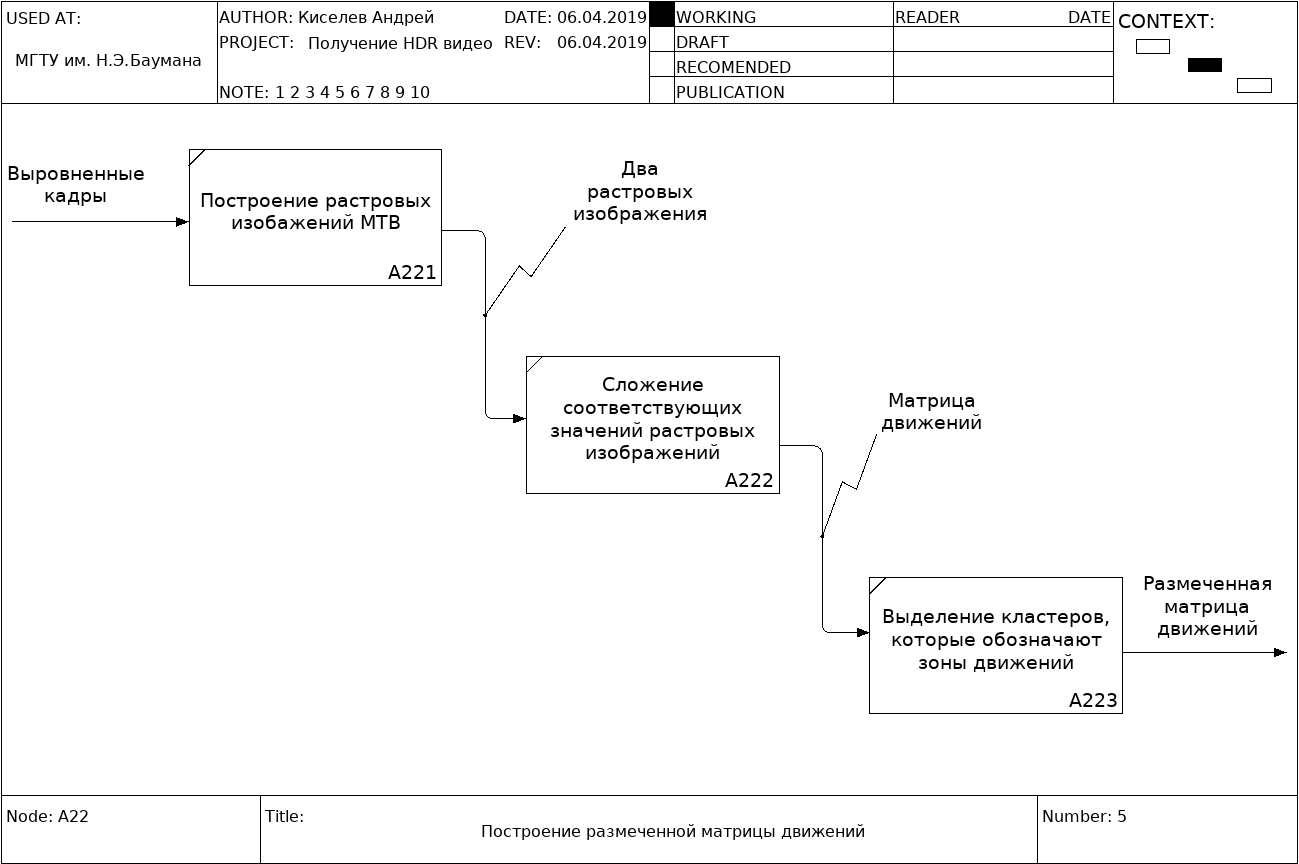
\includegraphics[width=1\textwidth]{img/05_A22.png}
	\caption{ IDEF0 диаграмма метода(A22)}
        \label{fig:A22}
        }
\end{figure}

\begin{figure}[ht!]
    \centering{
        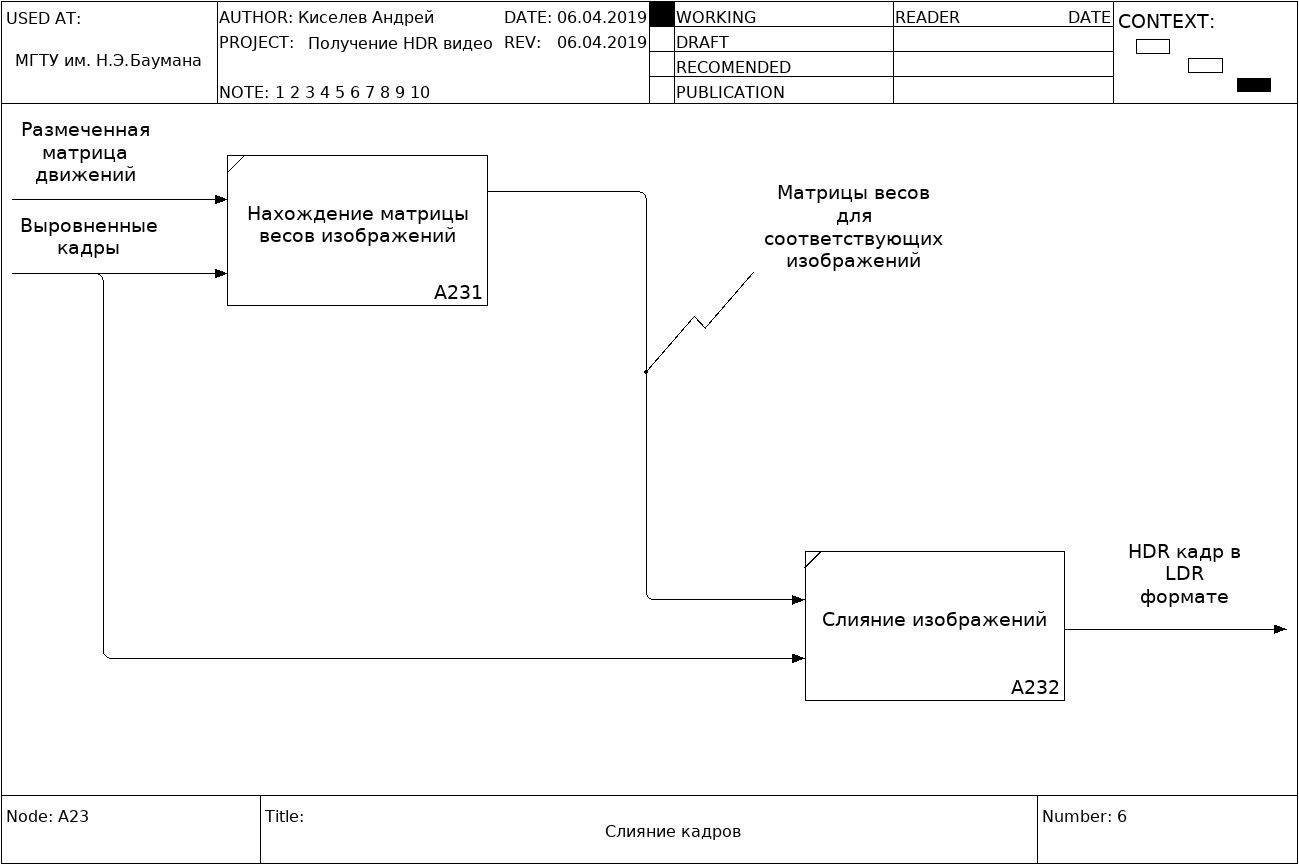
\includegraphics[width=1\textwidth]{img/06_A23.png}
	\caption{ IDEF0 диаграмма метода(A23)}
        \label{fig:A23}
        }
\end{figure}

